Una masa puntual \(m>0\) está sujeta a una varilla sin masa de longitud \(\ell>0\), que gira sin rozamiento. El ángulo \(\theta\), en radianes, se mide desde la vertical inferior. El momento de inercia es \(m\ell^2\), y el único par es \(-mg\ell\sin\theta\), con \(g>0\). La ley de movimiento iguala el momento de inercia por la aceleración angular al par neto.

Construya la EDO y su aproximación al sustituir \(\sin\theta\) por \(\theta\). Se acepta esa sustitución cuando el error de par relativo al módulo del par lineal no supera el \(1\%\):
\[
E(\theta)=\frac{|\theta-\sin\theta|}{|\theta|}\le0.01
\quad(\theta\ne0),\qquad E(0)=0.
\]
Use la desigualdad \(|\theta-\sin\theta|\le|\theta|^3/6\) para dar un intervalo angular garantizado. Calcule también \(E\) en \(0.20\) y \(0.30\) rad y decida si cada ángulo cumple el criterio. Explique a qué error se refiere la garantía y si permite, por sí sola, afirmar el mismo porcentaje para una trayectoria o un periodo.

\Needspace{7.8cm}
\begin{center}
\begin{minipage}{\linewidth}
\centering
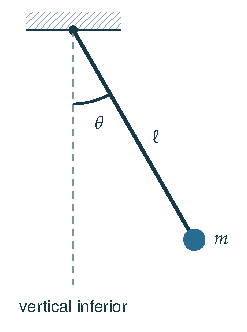
\includegraphics[width=4.69cm]{assets/M2-E0337-setup.pdf}\par
\smallskip{\small Referencia angular desde la vertical inferior.\par}
\end{minipage}
\end{center}
